Энергетические подходы стали популярны с публикацией прорывных работ по диффузионным порождающим 
моделям \cite{song2020score}. Ключевым отличием данного подхода является неявная работа с вероятностной
массой с использованием ненормированного потенциала. Такой подход позволяет исследователям адаптировать
физические модели для обучения и генерации данных. Так, например, процесс Ланжевена, описывающий
смещение частицы с случайной составляющей, может быть использован для генерации из распределения, заданного
исключительно потенциалом, без необходимости в численно затратной операции нормировки.

\textit{Определение:} \textbf{Энергетическими} подходами в машинном обучении 
называют класс статистических моделей, параметризующих вероятность 
состояния согласно энергии $E$:
\begin{equation}
    p(x) \sim \frac{\exp(-E(x))}{Z},
\end{equation}
где $Z=\int \exp(-E(x))$. 

На практике энергетический потенциал задается через параметрическую функцию $E(\mathbf{x},\theta,x)$, позволяющую
выполнять адаптацию модели с помощью методов градиентного спуска \cite{lecun2006tutorial}.

\textit{Определение:} \textbf{Диффузионные модели} \label{diffusion} представляют собой класс вероятностных моделей, 
использующих уравнение Ланжевена \ref{la} для генерации элементов $x$ из вероятного распределения $p$.

\begin{figure}[h]
    \centering
    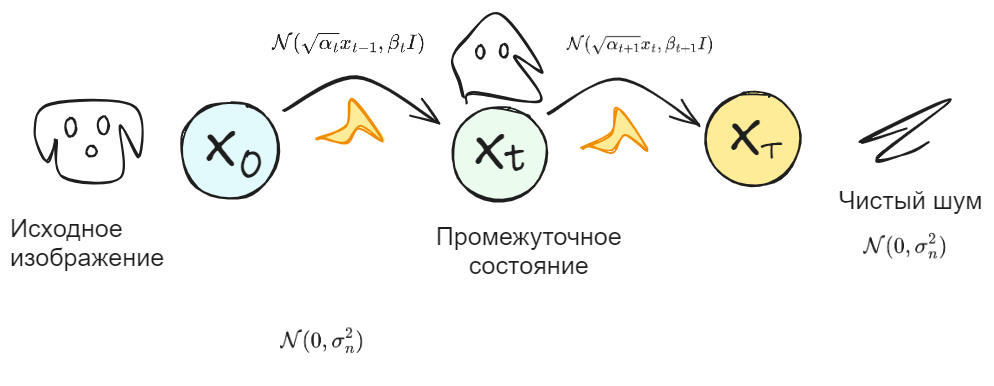
\includegraphics[width=0.5\textwidth]{assets/ml/generation/diffusion_1.excalidraw.png}
    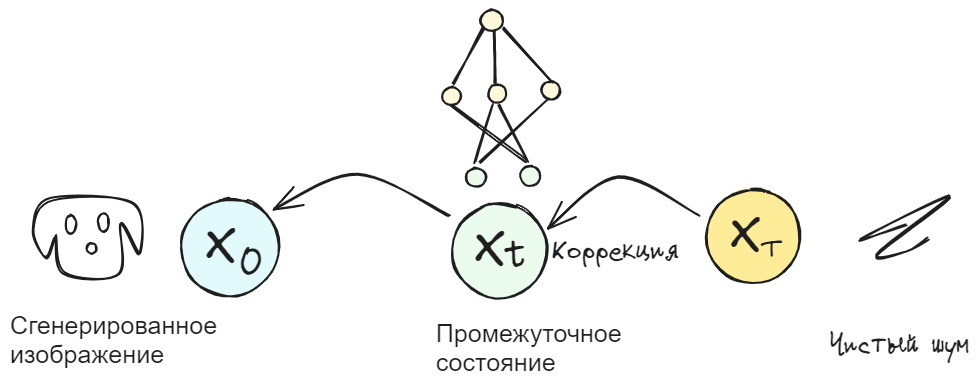
\includegraphics[width=0.5\textwidth]{assets/ml/generation/diffusion_2.excalidraw.png}
    \caption{Прямой процесс зашумления и обратный процесс коррекции ошибки \cite{stablediffusion}.}
    \label{sd_arch}
\end{figure}

В диффузионных моделях генерация выполняется в виде последовательных шагов, каждый из которых 
компенсирует ошибку начального изображения. Обучение исправлению ошибок выполняется путем предсказания 
шума между текущим и предыдущим шагом.

Прямым процессом диффузионной модели называется постепенное зашумление:
\begin{equation}
    x_t = \sqrt{1-\beta_t} x_{t-1} + \sqrt{\beta_t} z_t,
\end{equation}
где $z_t \sim \mathcal{N}(0,\mathbf{I})$. 
Тогда итоговое вероятностное распределение:
\begin{equation}
    q(x_{T}) = q(x_0)q(x_1|x_0) \dots q(x_T|x_{T-1}) =
    q(x_0) \mathcal{N}(x_1|\sqrt{1-\beta_t}x_0,\beta_1I)\dots
    \mathcal{N}(x_T|\sqrt{1-\beta_T}x_0,\beta_TI)
\end{equation}

В компактной форме:
\begin{equation}
    ln q(x_{T}) = ln q(x_0) - \sum_{t=1}^T \frac{1}{2\beta_t} \| x_t - \sqrt{1-\beta_t} x_{t-1} \|^2 + C
\end{equation}

Обратный процесс состоит в построении цепочки 
$\mathcal{N}(x_{t-1}|\mu(x_t,t),\Sigma(x_t,t))$, восстанавливающей элемент из шума:
\begin{equation}
    \begin{aligned}
        p_\theta(x_T) = \mathcal{N}(x_T|0,I);
        p_\theta(x_{t-1}|x_t) = \mathcal{N}(x_{t-1}|\mu_\theta(x_t,t), \Sigma_\theta(x_t,t))
    \end{aligned}
\end{equation}

Для введения параметрической модели используют нижнюю вариационную границу ELBO:
\begin{equation}
    \mathbb{E}_{x_0 \sim q} \ln p_\theta(x_0) \ge \mathrm{E} \ln p_\theta(x_T) - ln()
\end{equation}
Тогда функция ошибки запишется как:
\begin{equation}
    \begin{aligned}
        &L(\theta) = - \sum_{t=1}^T\mathbb{E}_{x_{t-1},x_t \sim q} \left[-ln p_\theta(x_{t-1|x_t}\right] + \\
        &+ \mathbb{E}_{x_0 \sim q} \mathbf{D}_{KL}(q(x_T|x_0) \parallel p_\theta (x_T))
    \end{aligned}
\end{equation}

На практике функция ошибки упрощается до предсказания шума:
\begin{equation}
    \mathrm{E}_{x_0 \sim q; z\sim \mathcal{N}(0,I)} 
    \left[ \| \varepsilon_\theta(x_t,t) -z \|^2\right]
\end{equation}


